\iffalse
\documentclass[12pt]{article}
\usepackage{graphicx}
\usepackage{amsmath}
\usepackage{mathtools}
\usepackage{gensymb}

\newcommand{\mydet}[1]{\ensuremath{\begin{vmatrix}#1\end{vmatrix}}}
\providecommand{\brak}[1]{\ensuremath{\left(#1\right)}}
\providecommand{\norm}[1]{\left\lVert#1\right\rVert}
\newcommand{\solution}{\noindent \textbf{Solution: }}
\newcommand{\myvec}[1]{\ensuremath{\begin{pmatrix}#1\end{pmatrix}}}
\let\vec\mathbf

\begin{document}
\begin{center}
\textbf\large{CHAPTER-11 \\ CIRCLES}

\end{center}
\section*{Excercise 11.1}

Q4.Find the equation of the circle with centre $(1,1)$ and radius $\sqrt{2}$.

\solution
\fi
Given
\begin{align}
	\vec{c} &= \myvec{1\\1} \text{ and } r = \sqrt{2},
	\\
	\vec{u}&=\vec{-c}
	 = \myvec{-1\\-1}\\
	 \\
	f &= \norm{\vec{u}}^2 - r^2
	  =0	
\end{align}
Thus, the equation of circle is 
\begin{align}
	\norm{\vec{x}}^2 -2\myvec{1&1}\vec{x} = 0       		       
\end{align}	
See Fig. 
\ref{fig:chapters/11/11/1/4/Fig1}.
\begin{figure}[!h]
	\begin{center} 
	  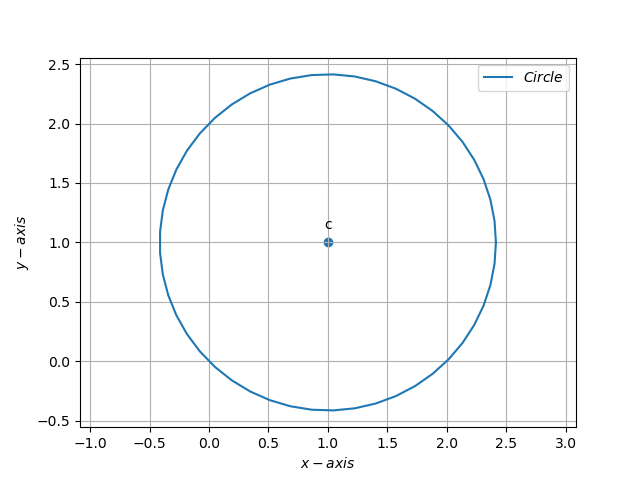
\includegraphics[width=\columnwidth]{chapters/11/11/1/4/figs/circ.png}
	\end{center}
\caption{}
\label{fig:chapters/11/11/1/4/Fig1}
\end{figure}
